\subsection{Layer 5, 6, 7 (Session, Presentation, Application)}
\subsection*{Aufgaben}
\begin{itemize}
	\item Session erstellen und halten
	\item Regelung der Session, Restart, Exchange, Idle
	\item Format und Präsentation der Daten
	\item Verschlüsselung und Komprimierung der Daten
	\item Anwendungsspezifische Informationen
\end{itemize}
\textbf{Protokolle:} HTTP/HTTPS, FTP, Telnet/SSH, DHCP, DNS, SMTP, POP, IMAP

\subsection*{DNS (Port 53, UDP)}
Um zu einer Domain die passende IP-Adresse zu finden.
Typische DNS-Server: 8.8.8.8

\begin{figure}[H]
	\centering
	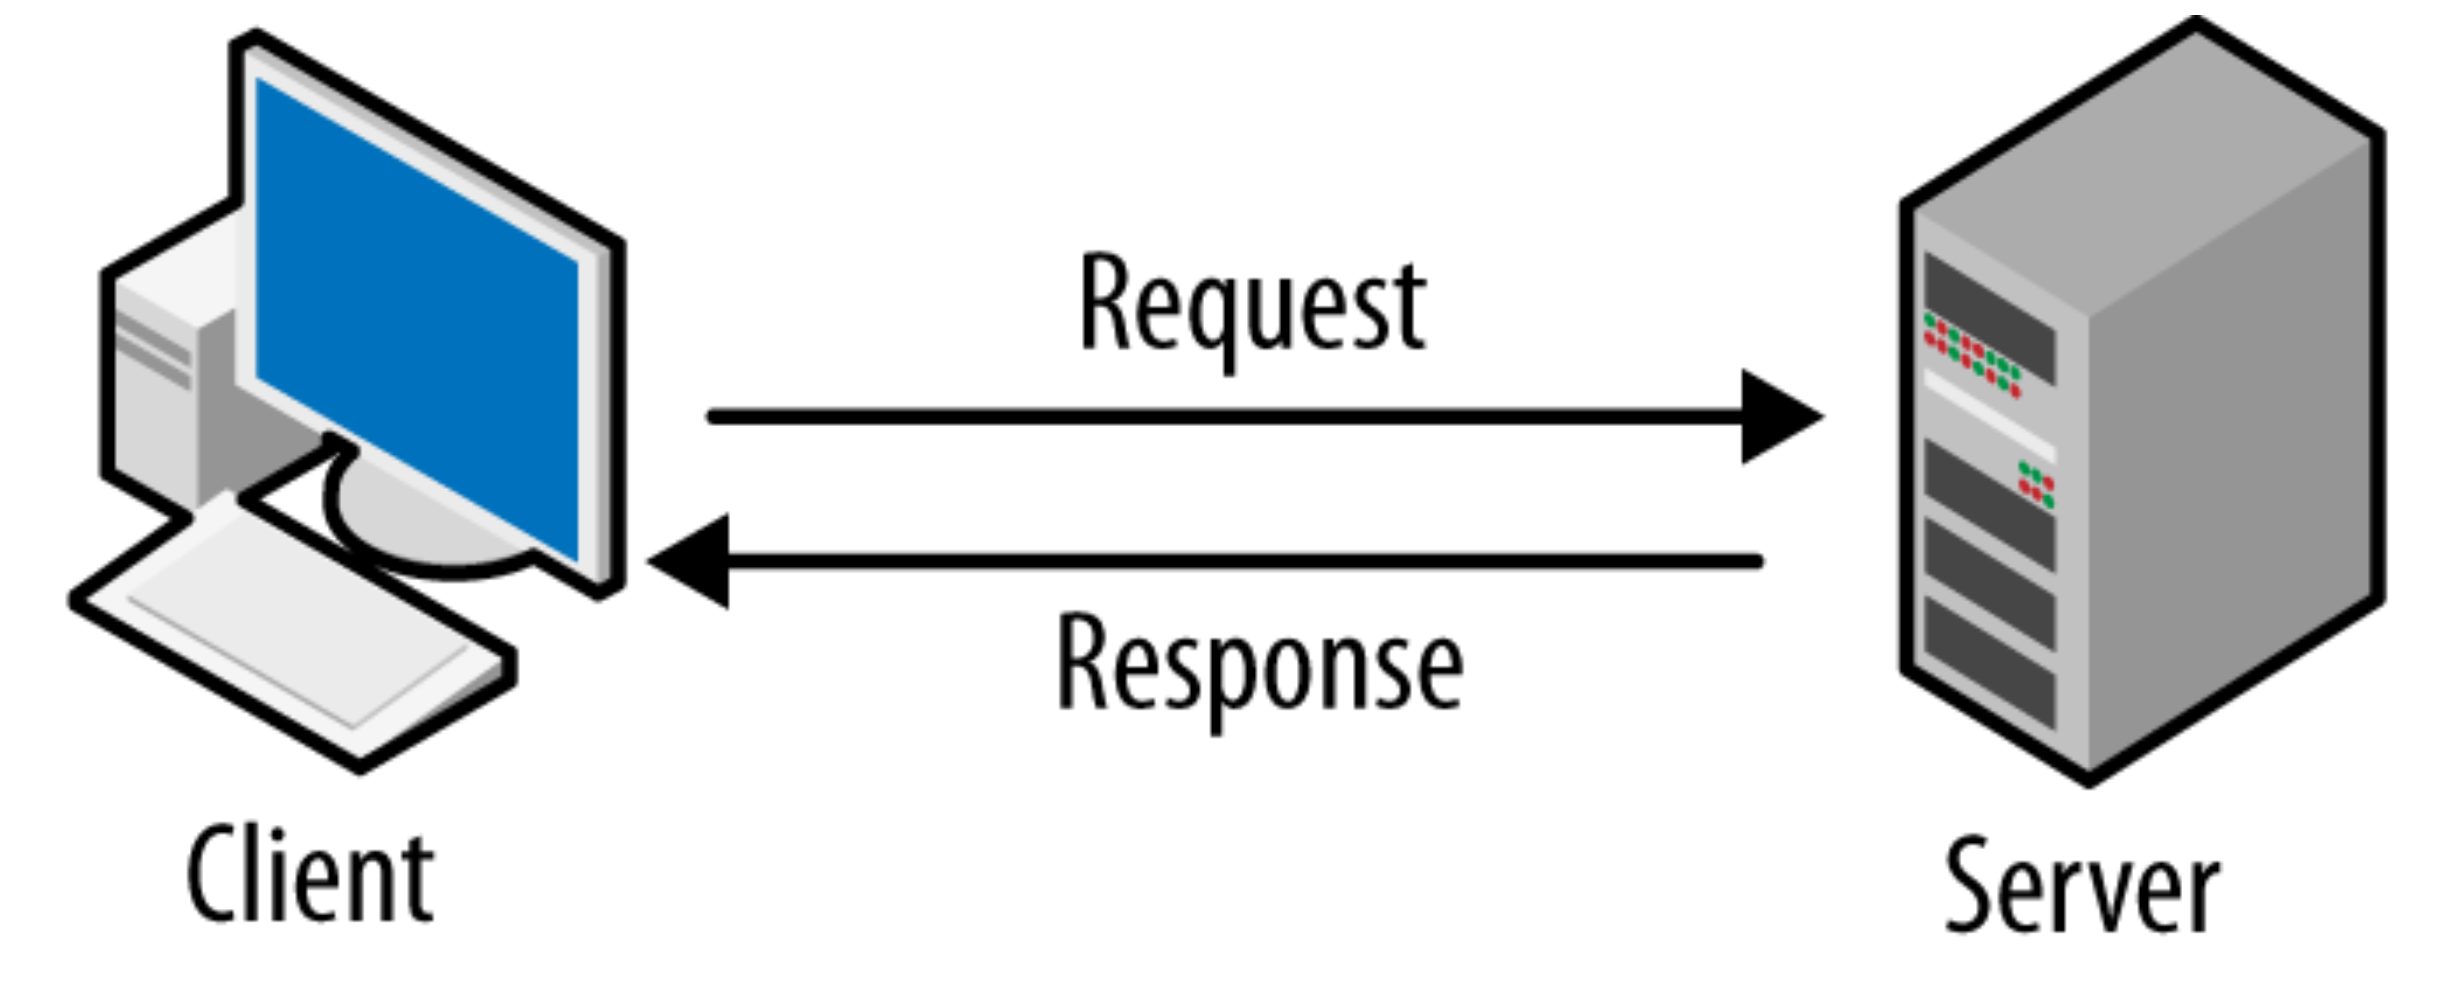
\includegraphics[width=0.8\linewidth]{figures/request_response.png}
	\caption{Request/Response Modell}
\end{figure}

\subsection*{Einträge}
A ... IPv4-Endgerät \\
AAAA ... IPv6-Endgerät \\
MX ... Mail-Server

\subsection*{Hierarchisches DNS-Modell}
\begin{figure}[H]
	\centering
	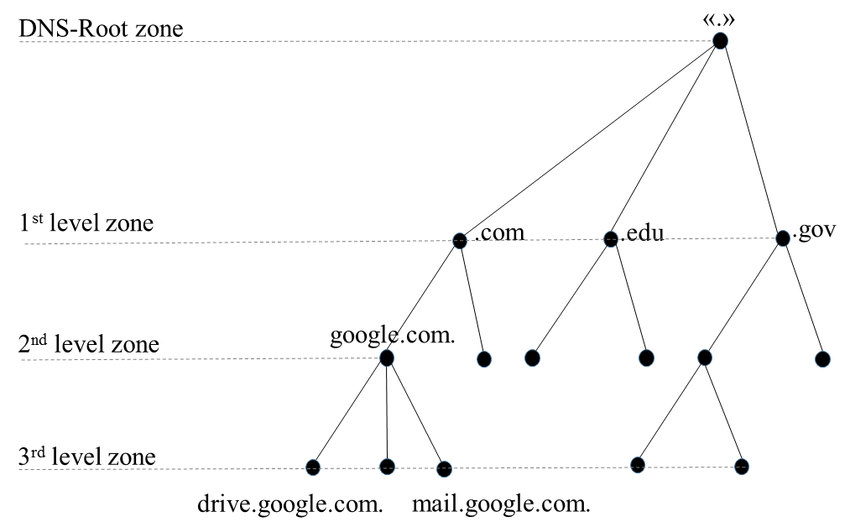
\includegraphics[width=0.8\linewidth]{figures/dns_hierarchy.png}
	\caption{DNS-Hierarchie}
\end{figure}
Falls der DNS-Server keinen Eintrag findet, wird das Paket weitergeleitet. Der Client speichert die erhaltenen DNS-Einträge.

\subsection*{DHCP (Port 67/68, UDP)}
Die Hosts erhalten dynamisch eine IP-Konfiguration (IP-Adresse, Subnetzmaske, Default Gateway, DNS-Server, Lease Time,...).

\begin{figure}[H]
	\centering
	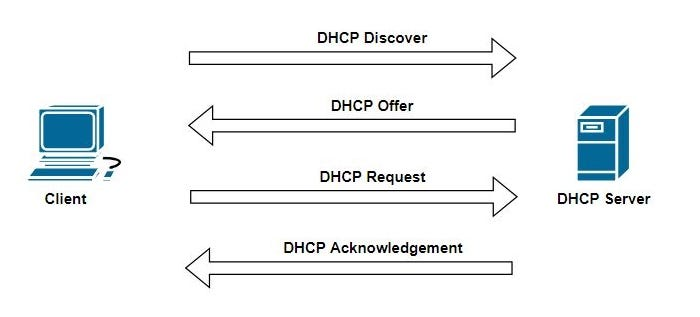
\includegraphics[width=0.8\linewidth]{figures/dhcp_handshake.jpg}
	\caption{DHCP-Handshake}
\end{figure}
DHCP-Discover ... Broadcast \\
DHCP-Offer ... Unicast \\
DHCP-Request ... Broadcast \\
DHCP-ACK ... Unicast \\ 
\textbf{Achtung:} DHCP-Spoofing

\subsection*{HTTP/HTTPS (Port 80/443, TCP)}
\begin{figure}[H]
	\centering
	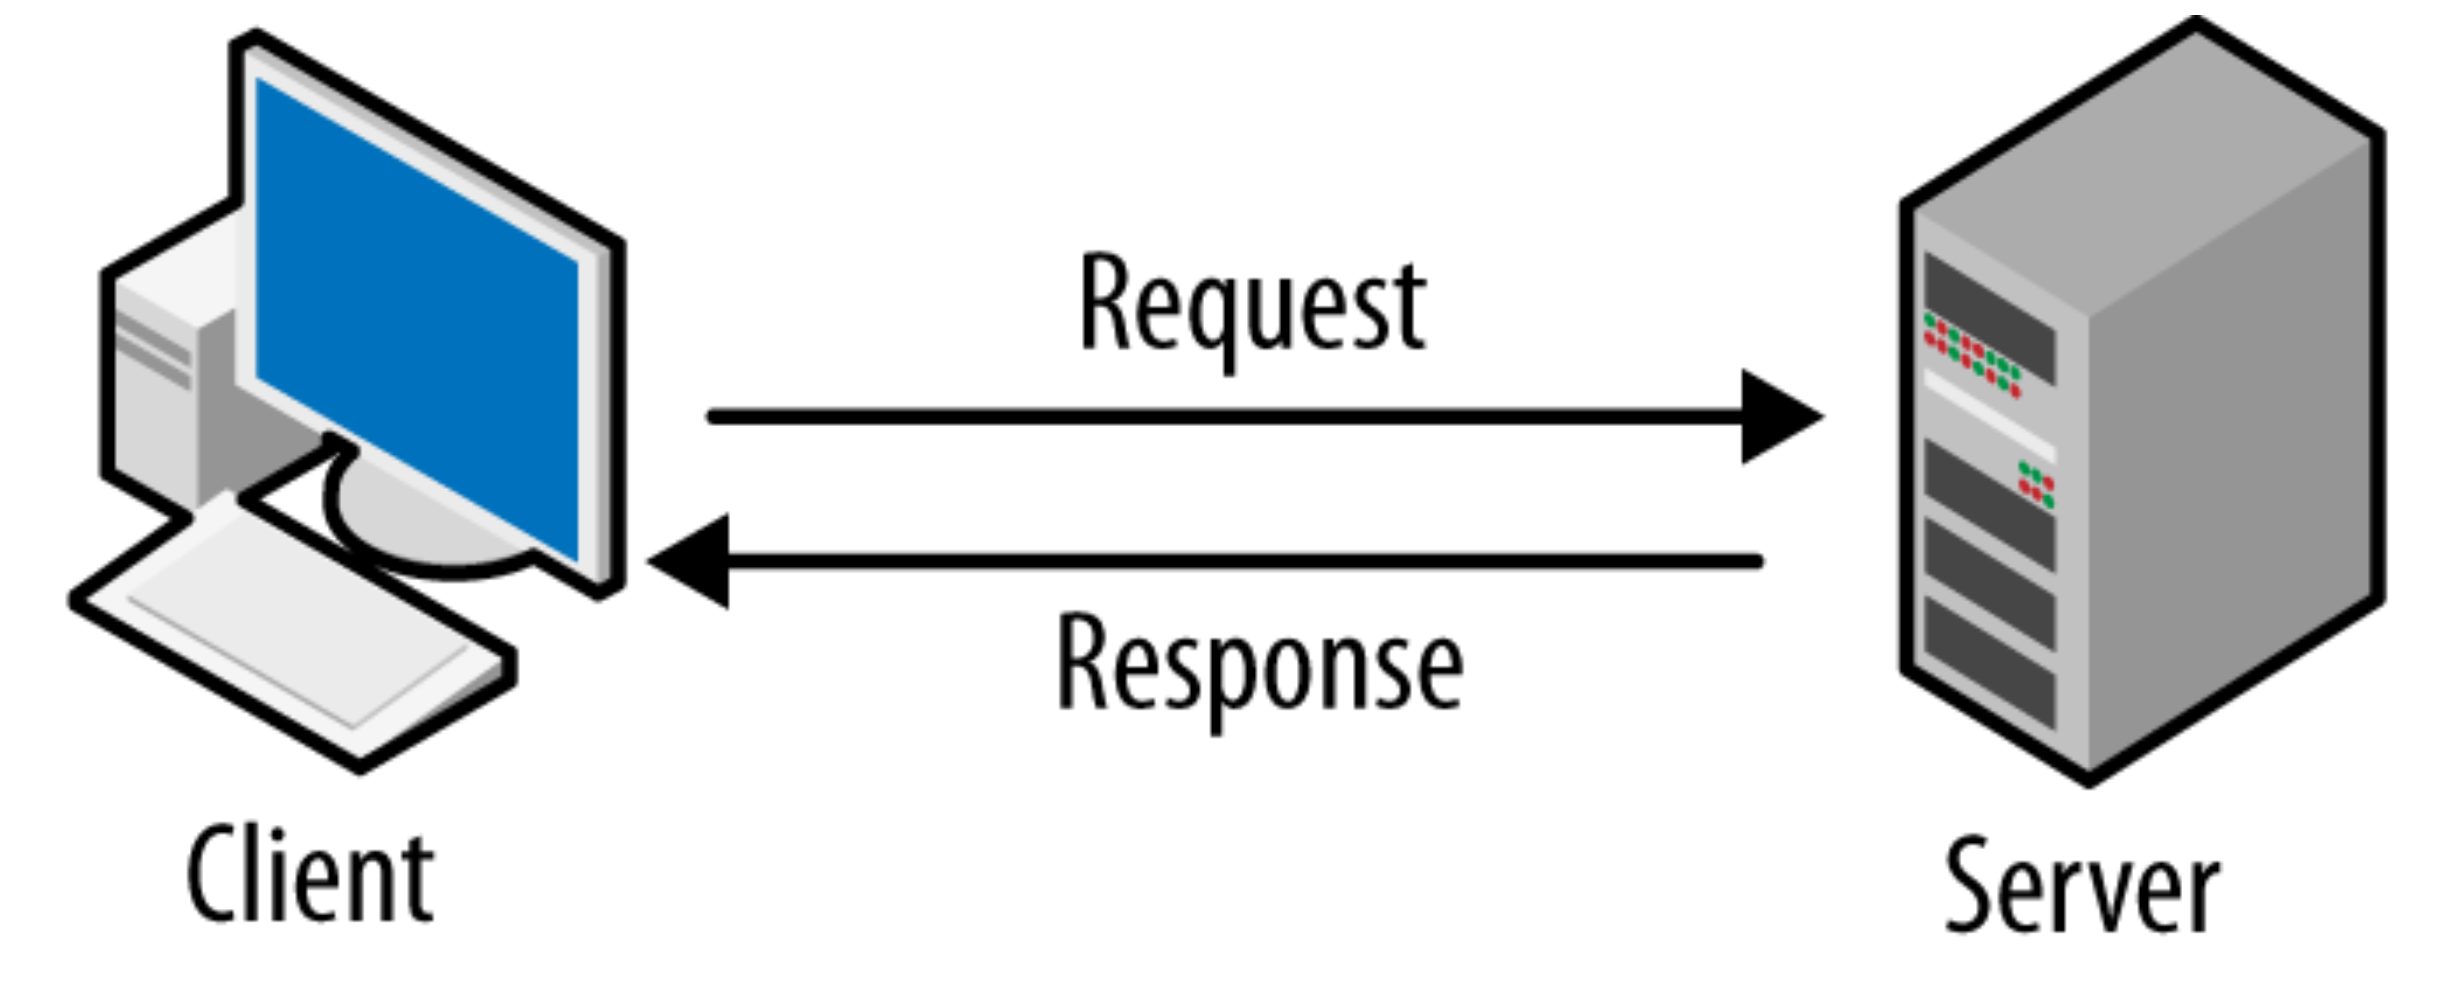
\includegraphics[width=0.8\linewidth]{figures/request_response.png}
	\caption{Request/Response Modell}
\end{figure}

\begin{table}[H]
	\begin{tabular}{c|c|c|c}
		URL: & https:// & www.google.com/ & index.html \\
		\hline
		& Protokoll & Domain IP-Adresse (DNS) & Ordnerstruktur, Datei
	\end{tabular}
\end{table}

\subsection*{Befehle}
Get, Post, Put, Delete,...

Bei HTTP ist alles im Klartext. \\
Bei HTTPS wird zusätzlich mit SSL/TLS verschlüsselt.

\subsection*{E-Mail}
\begin{table}[H]
	\begin{tabular}{c|c|c|c}
		E-Mail-Adresse: & name & @ & gmail.com \\
		\hline
		& Benutzername & & Domain
	\end{tabular}
\end{table}

\subsection*{SMTP (Port 25, TCP)}
Senden von Emails. Wird zum Senden von Mails und dem Weiterleiten zum Zielserver benutzt. SMTP kann zusätzlich Feedback geben (z.b. Ziel nicht erreichbar,...).

\subsection*{POP (Port 110, TCP)}
Empfangen von E-Mails. Man erhält vom Server das Original. Die Mail wird am Server gelöscht (Vorteil: Speicherplatz, Security).

\subsection*{IMAP (Port 143, TCP)}
Empfangen von E-Mails. Man erhält vom Server eine Kopie. Das Original bleibt am Server gespeichert (Vorteil: Verbindung mit mehreren Geräten ist praktisch, Backup).
